%=======================02-713 LaTeX template, following the 15-210 template==================
%
% You don't need to this template
%
\documentclass[11pt]{article}
\usepackage{amsmath,amssymb,amsthm}
\usepackage{graphicx}
\usepackage[margin=1in]{geometry}
\usepackage{fancyhdr}
\usepackage{multicol}
\usepackage{mathtools}
\usepackage{float}
\setlength{\parindent}{0pt}
\setlength{\parskip}{5pt plus 1pt}
\setlength{\headheight}{13.6pt}
\newcommand\tab[1][1cm]{\hspace*{#1}}
\newcommand\question[2]{\vspace{.25in}\hrule\textbf{#1: #2}\vspace{.5em}\hrule\vspace{.10in}}
\renewcommand\part[1]{\vspace{.10in}\textbf{(#1)}}
\newcommand\header[3]{\begin{center}{#1} \\ {#2} \\ \textbf{#3} \end{center}}

\begin{document}\raggedright
	
	\header
	{BLG 433E Computer Communications, Spring 2018}
	{Homework \#2}
	{Due Dec 09, 2018}
	
	\begin{center}
		Kadir Emre Oto \\
		(150140032)
	\end{center}
	
	\question{1}{DHCP (20 Points)}
	
	Use Wireshark to investigate DHCP protocol on your computer while getting an IP address from a DHCP server. Show the communication between your computer and the DHCP server with a sequence diagram and briefly describe each of the four messages seen in the diagram. (Hint: You can take on/off the airplane mode if you are not able to see discover and offer messages.)
	
	\begin{figure}[h]
		\centering
		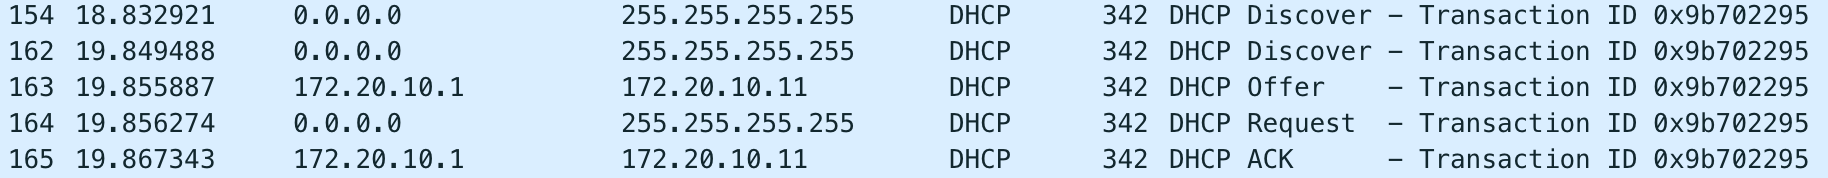
\includegraphics[width=1\linewidth]{dhcp}
		\caption{DHCP Packet Diagram captured by Wireshark}
	\end{figure}
	
	As we can see in the Figure 1, there are four steps in Dynamic Host Configuration Protocol (DHCP) to lease for various DHCP options like IP addresses. 
	
	\begin{enumerate}
		\item \textbf{DHCP Discover:} The client sends a DHCP server a request to lease an IP address.
		\item \textbf{DHCP Offer:} The DPCP servers offer an IP address to the client.
		\item \textbf{DHCP Request:} The client sends DHCP servers a request to lease one of IP adresses that are offered by DHCP servers.
		\item \textbf{DHCP ACK:} The requested DHCP server sends the client an acknowledge for requsted IP address, and updates its DHCP database. After now, the client can start communications over the network.
	\end{enumerate}
	
	\clearpage
	
	\question{2}{Video and Voice Traffic (20 Points)}
	
	Try to capture a video traffic and a voice traffic over Wireshark on your computer. You can use one of the video/music sharing platforms. Please, state the protocols used by investigating packet headers. Is there any retransmission during the sessions using TCP or UDP protocols? Please, indicate and interpret the results.
	
	In order to capture a video traffic, I used very popular video streaming website, netflix. This website broadcasts the videos by using Transmission Control Protocol (TCP). As we can see in Figure 2, some packets were retransmitted by the server (i.e. frame no 43767). The reason can be the latency in the acknowledge (ACK) packet from the client, and the server could think that the frame was not sent properly, and send the packet again. 
	
	In order to capture a voice traffic, I used an application, Discord. It allows the users to establish a voice chat by using User Datagram Protocol (UDP) (Figure 3). There is no retransmission during the session. 
	
	\begin{figure}[H]
		\centering
		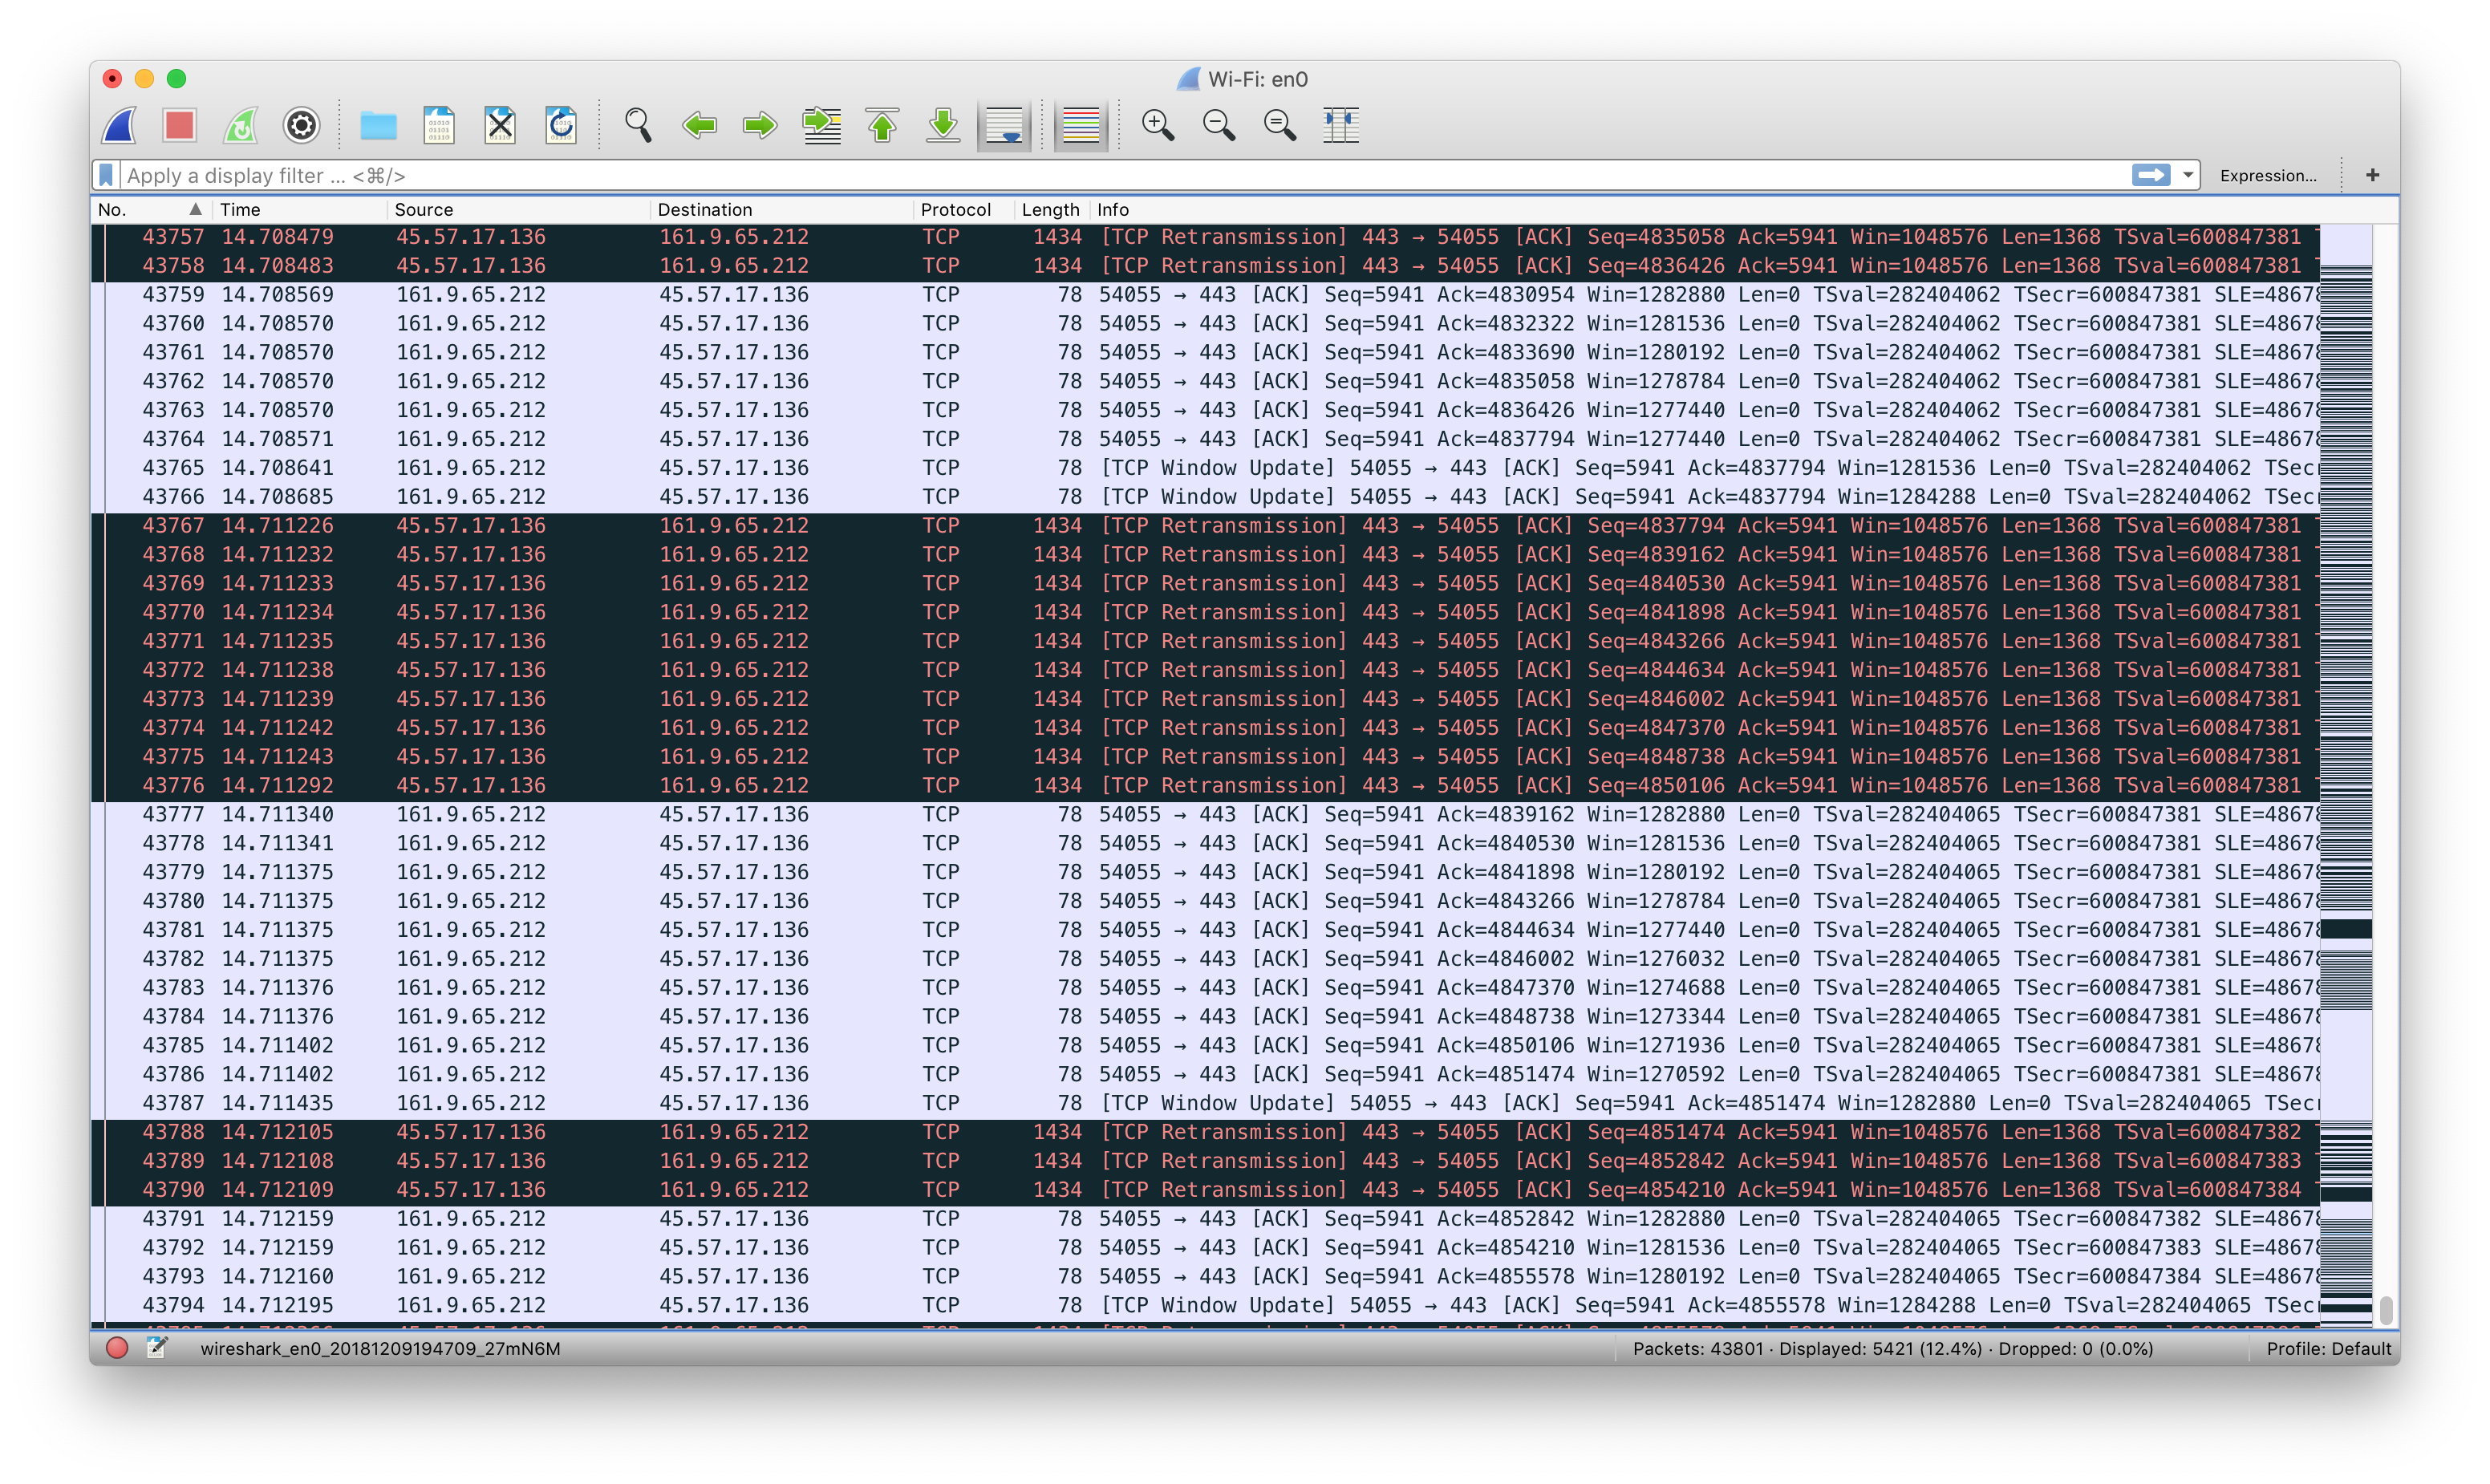
\includegraphics[width=1\linewidth]{video_stream}
		\caption{The Video Stream Frames captured by Wireshark}
	\end{figure}

	\begin{figure}[H]
		\centering
		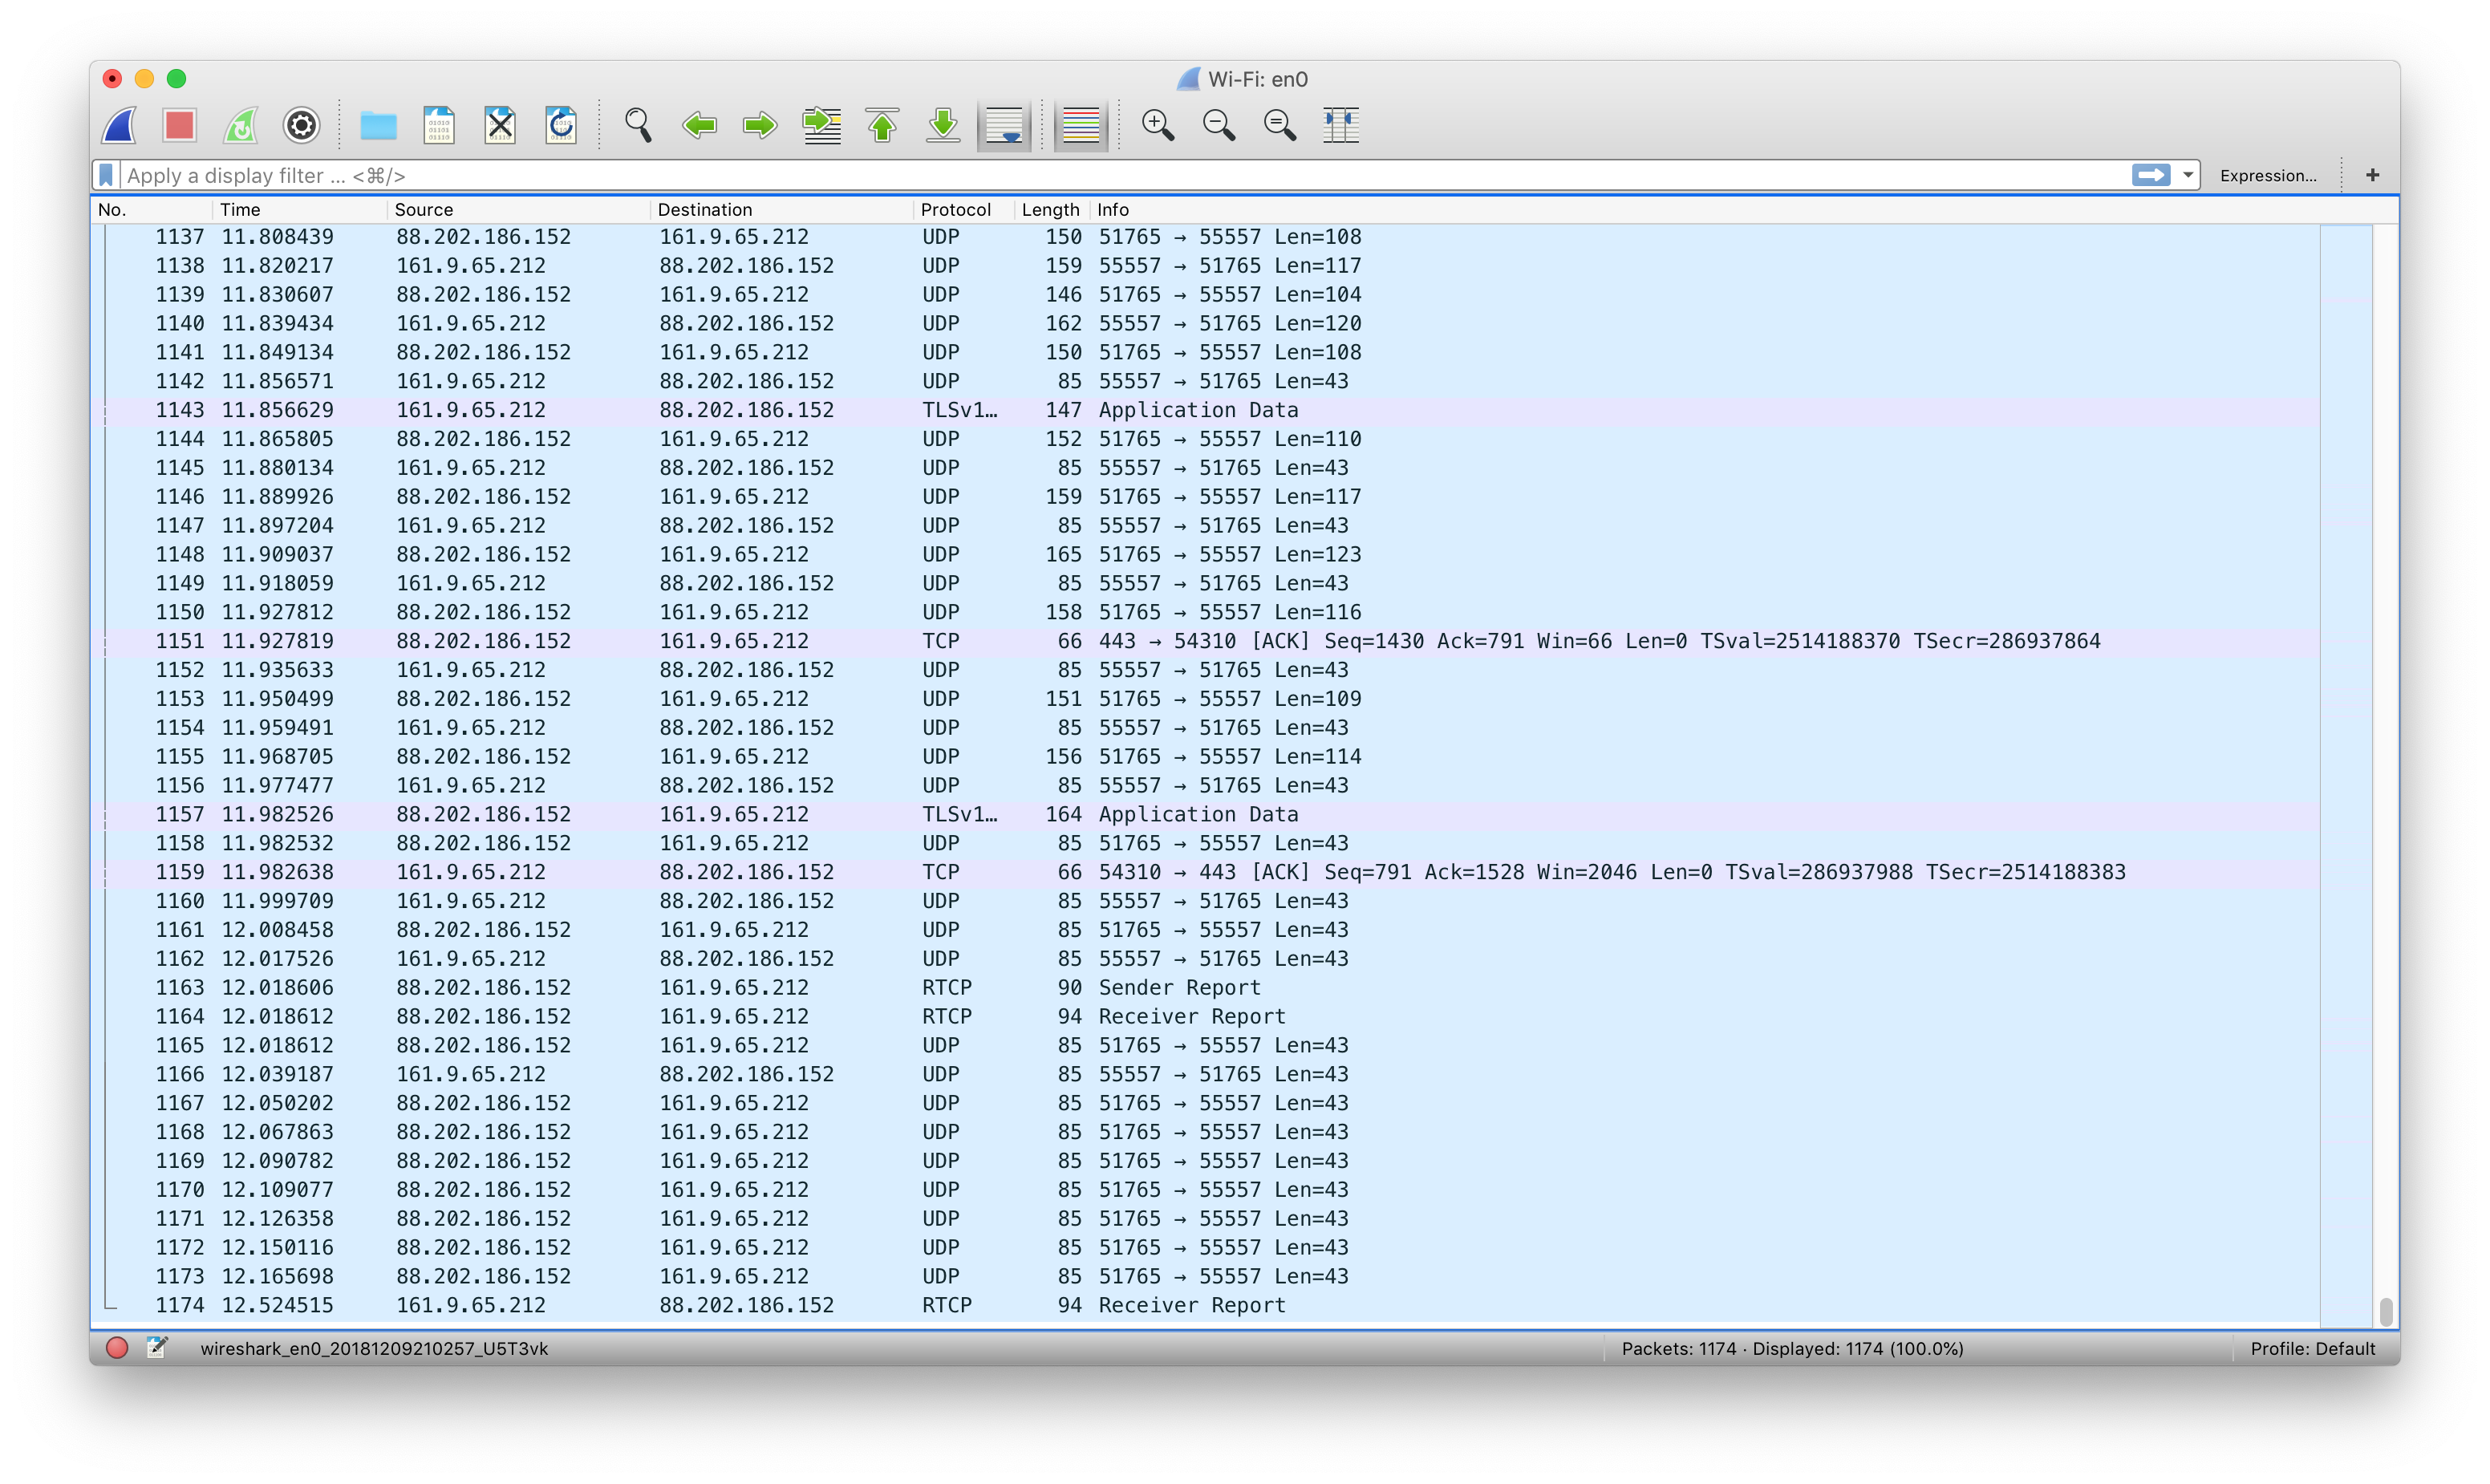
\includegraphics[width=1\linewidth]{voice_stream}
		\caption{The Voice Stream Frames captured by Wireshark}
	\end{figure}
	

	
	\question{3}{Throughput, RTT, and Window Size (20 Points)}

	Try to capture a session that uses TCP protocol while listening to music or visiting a webpage. Using "Statistics" pane in Wireshark, Provide drawings for Throughput, RTT, and Window Size parameters over the session. Interpret the figures considering/referring TCP congestion control mechanism.
	
	The drawings for Throughput, RTT, and Window Size parameters are provided in Figures 4, 5, 6, 7, 8, and 9.
	
	\begin{figure}[H]
		\centering
		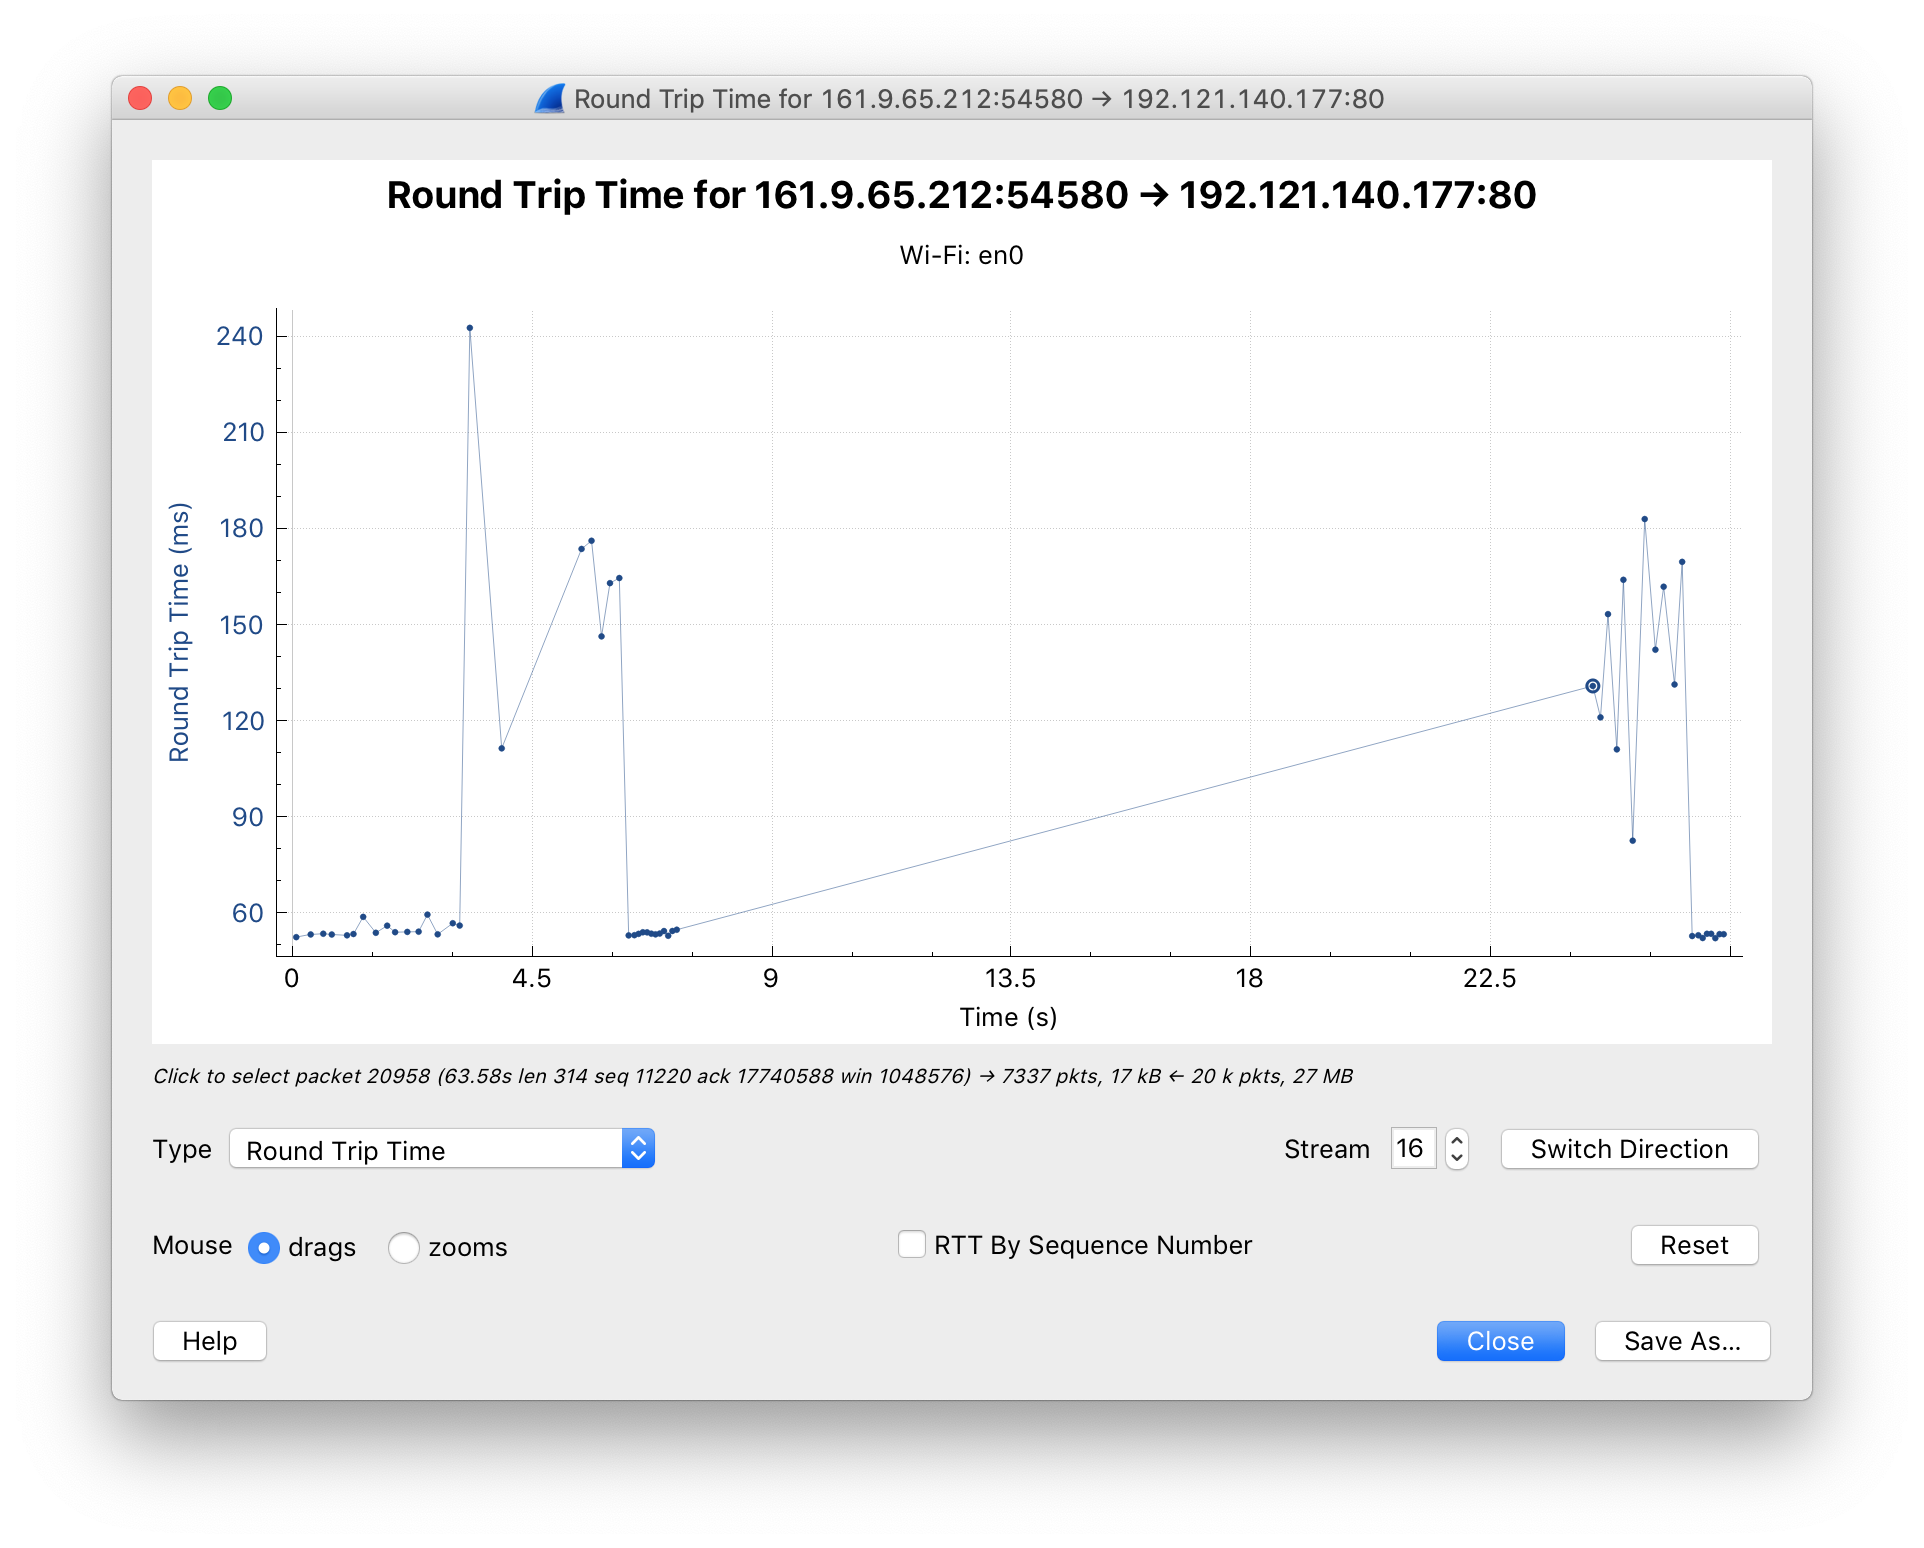
\includegraphics[width=0.7\linewidth]{rtt1}
		\caption{Round Trip Time for client to server}
	\end{figure}

	\begin{figure}[H]
		\centering
		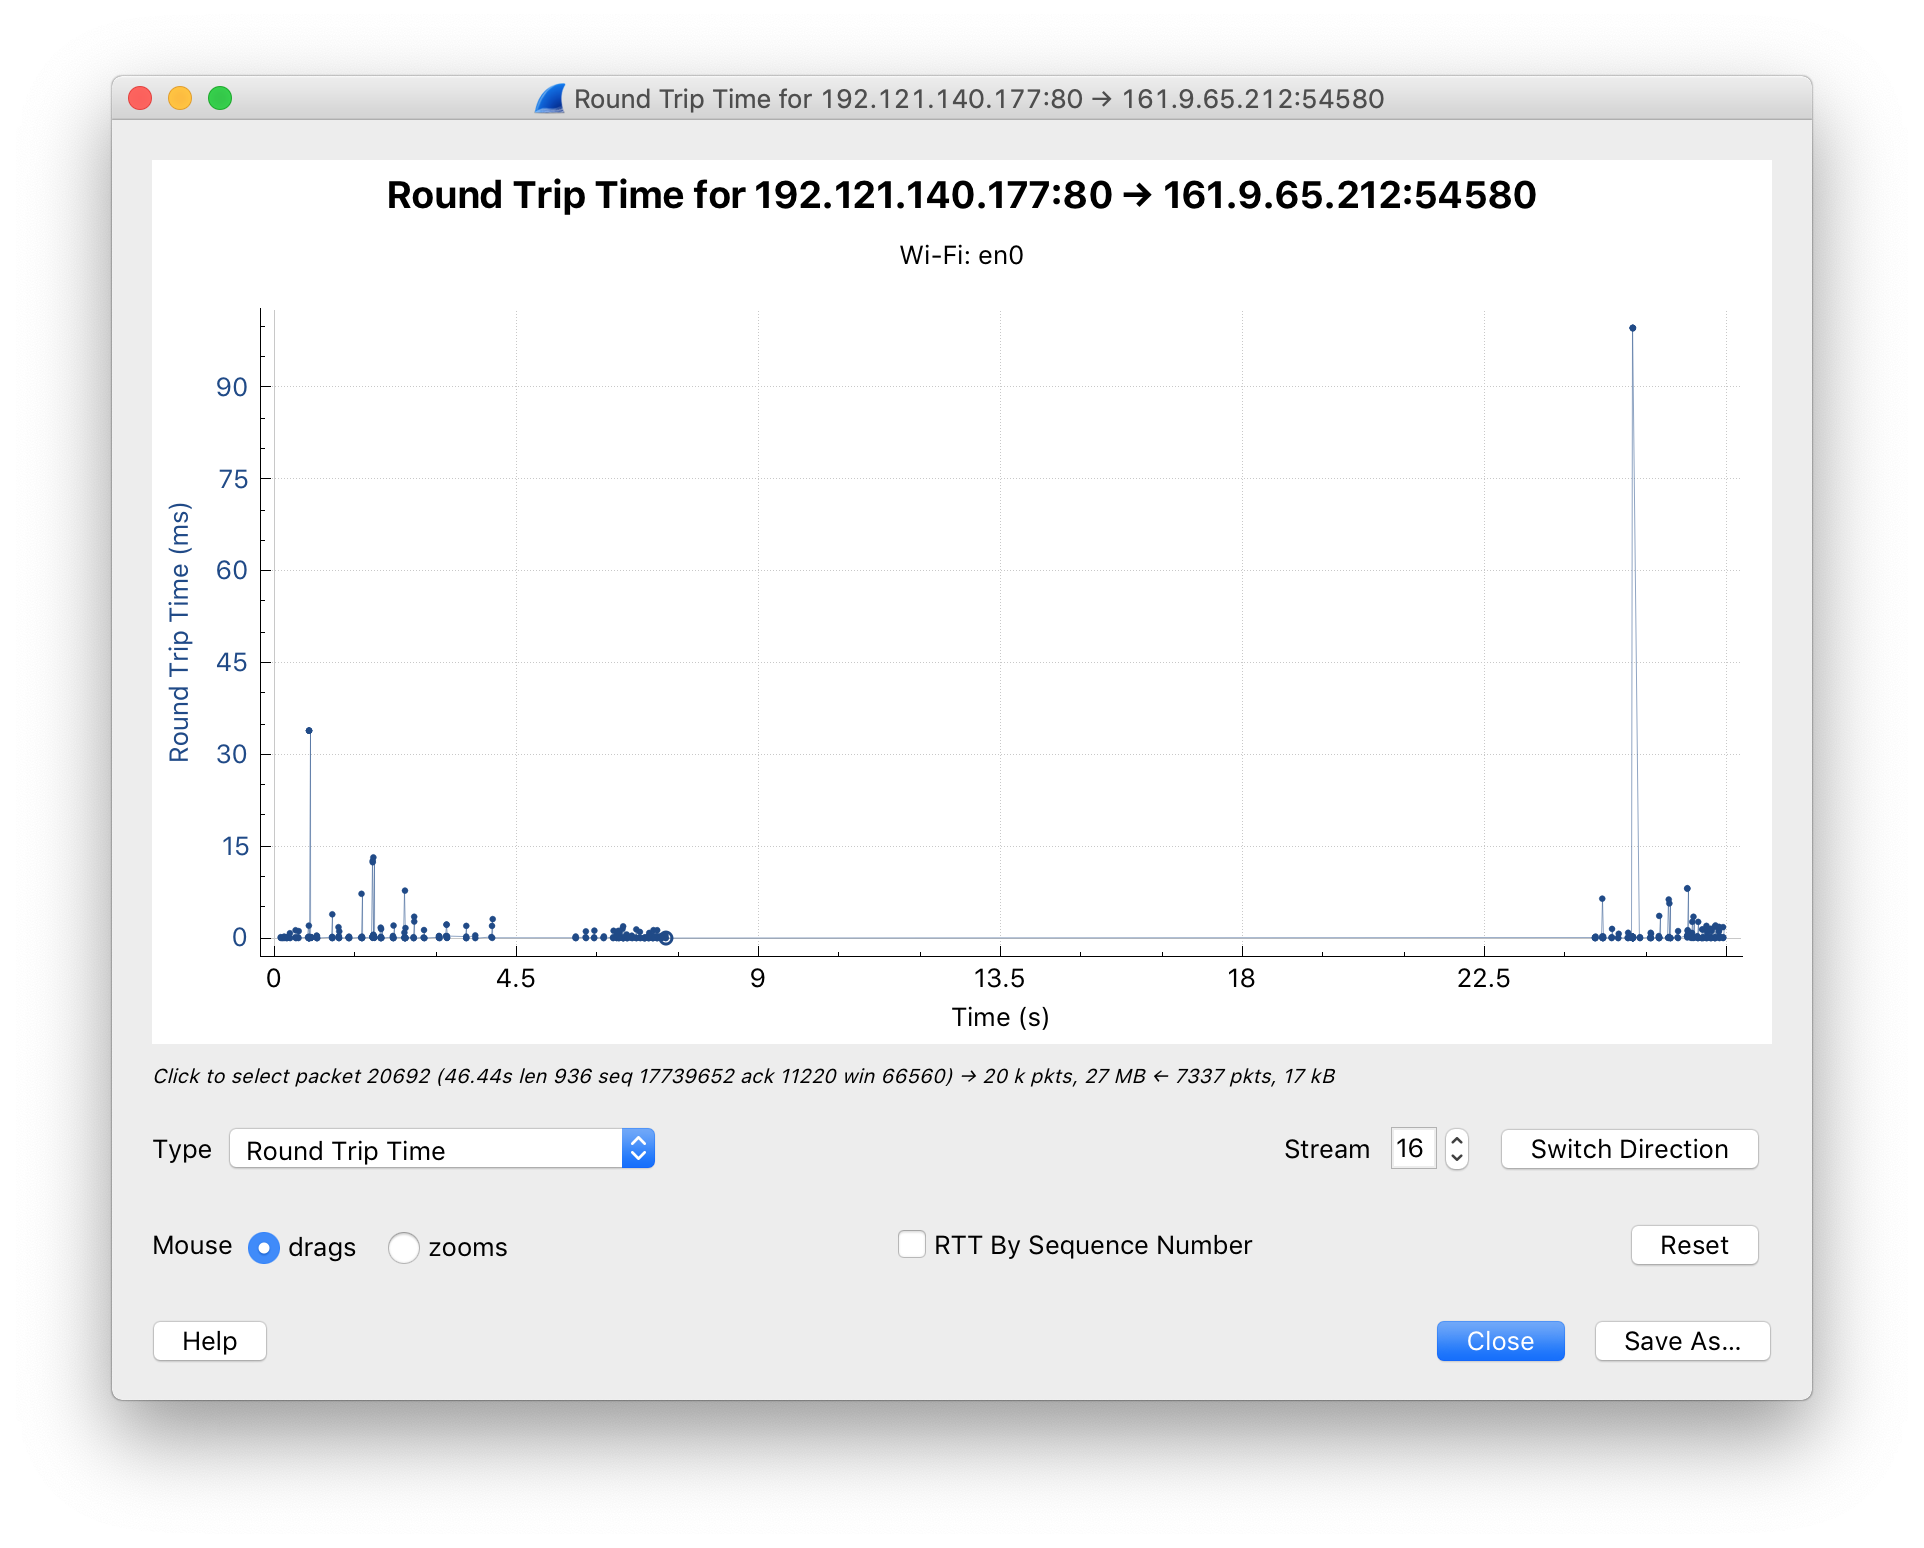
\includegraphics[width=0.7\linewidth]{rtt2}
		\caption{Round Trip Time for server to client}
	\end{figure}

	\begin{figure}[H]
		\centering
		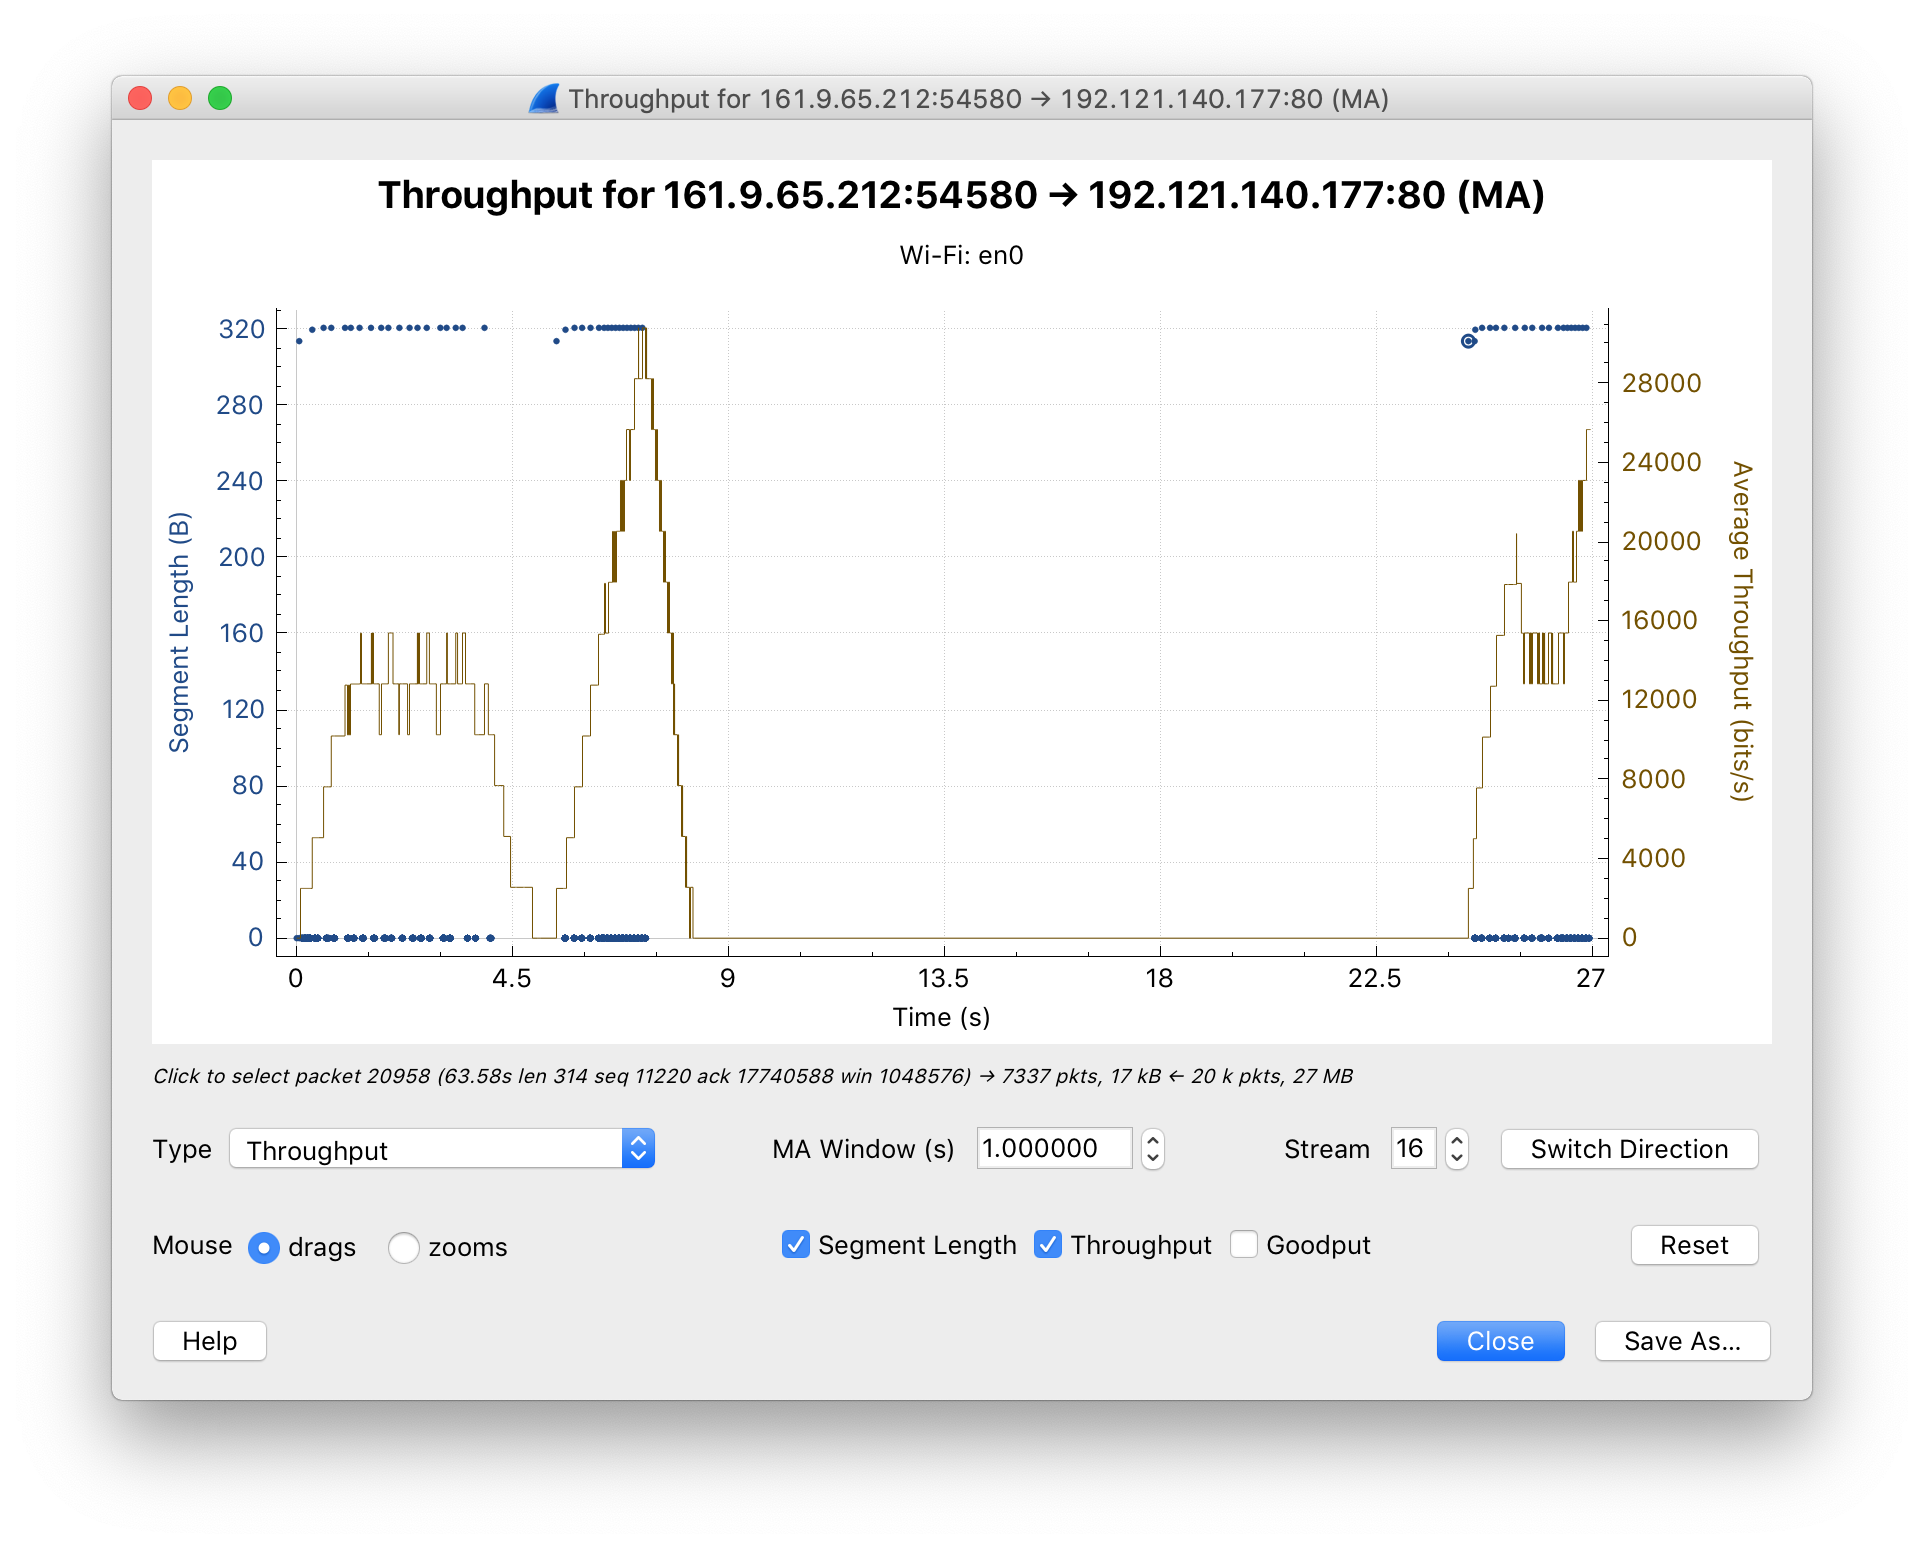
\includegraphics[width=0.7\linewidth]{throughput1}
		\caption{Throuhput for client to server}
	\end{figure}
	
	
	\begin{figure}[H]
		\centering
		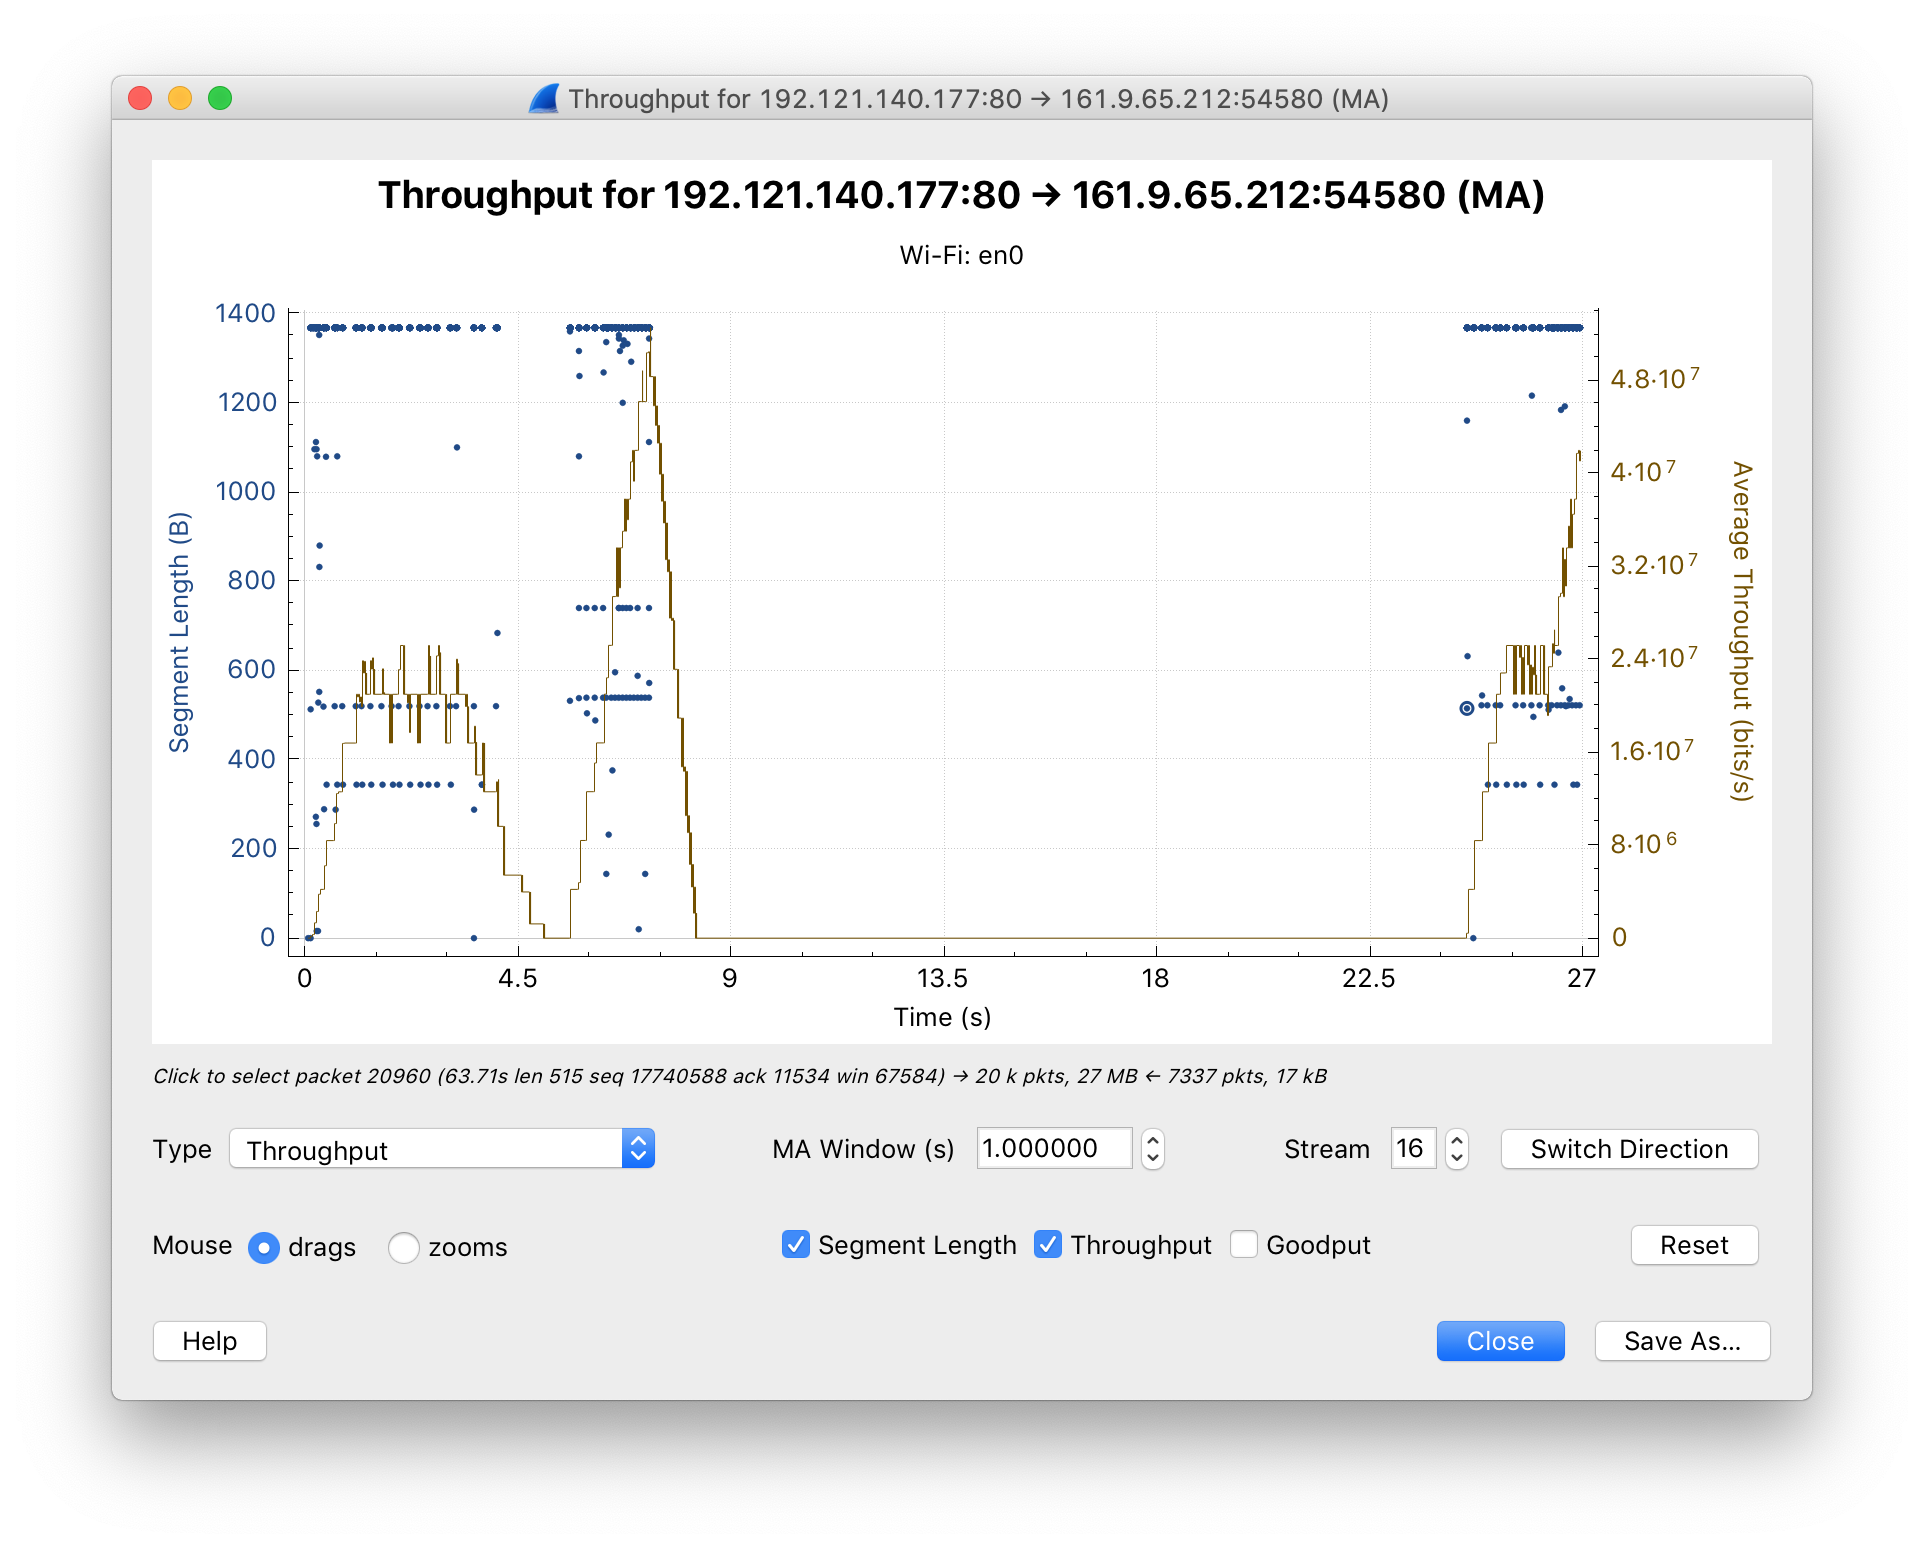
\includegraphics[width=0.7\linewidth]{throughput2}
		\caption{Throuhput for server to client}
	\end{figure}

	\begin{figure}[H]
		\centering
		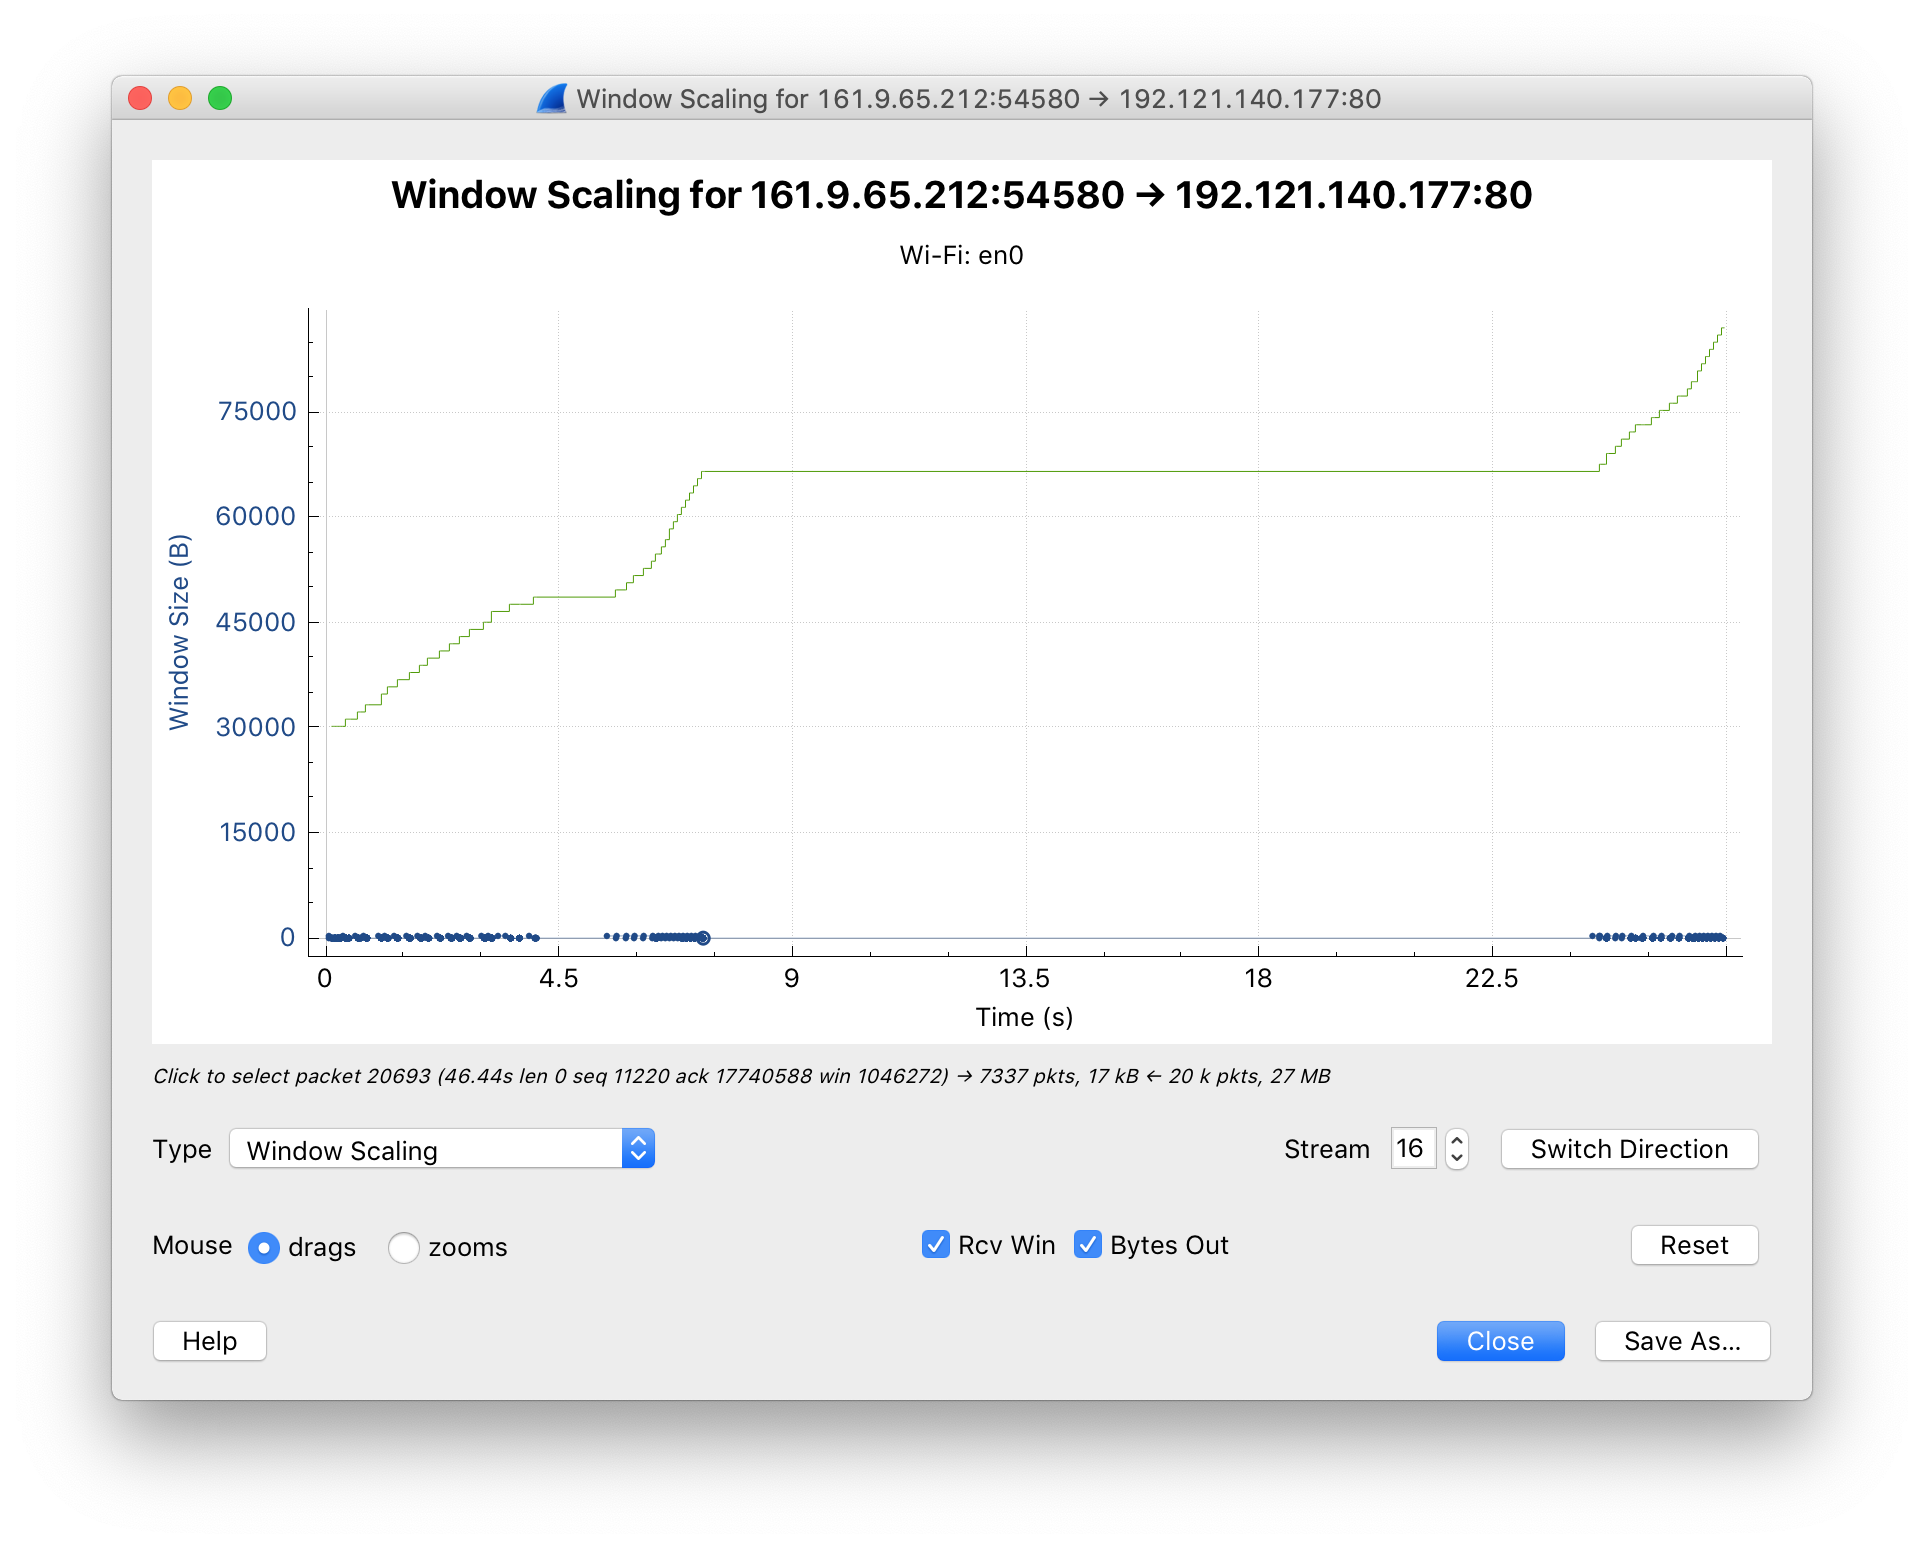
\includegraphics[width=0.7\linewidth]{window_scale1}
		\caption{Window Scaling for client to server}
	\end{figure}
	
	
	\begin{figure}[H]
		\centering
		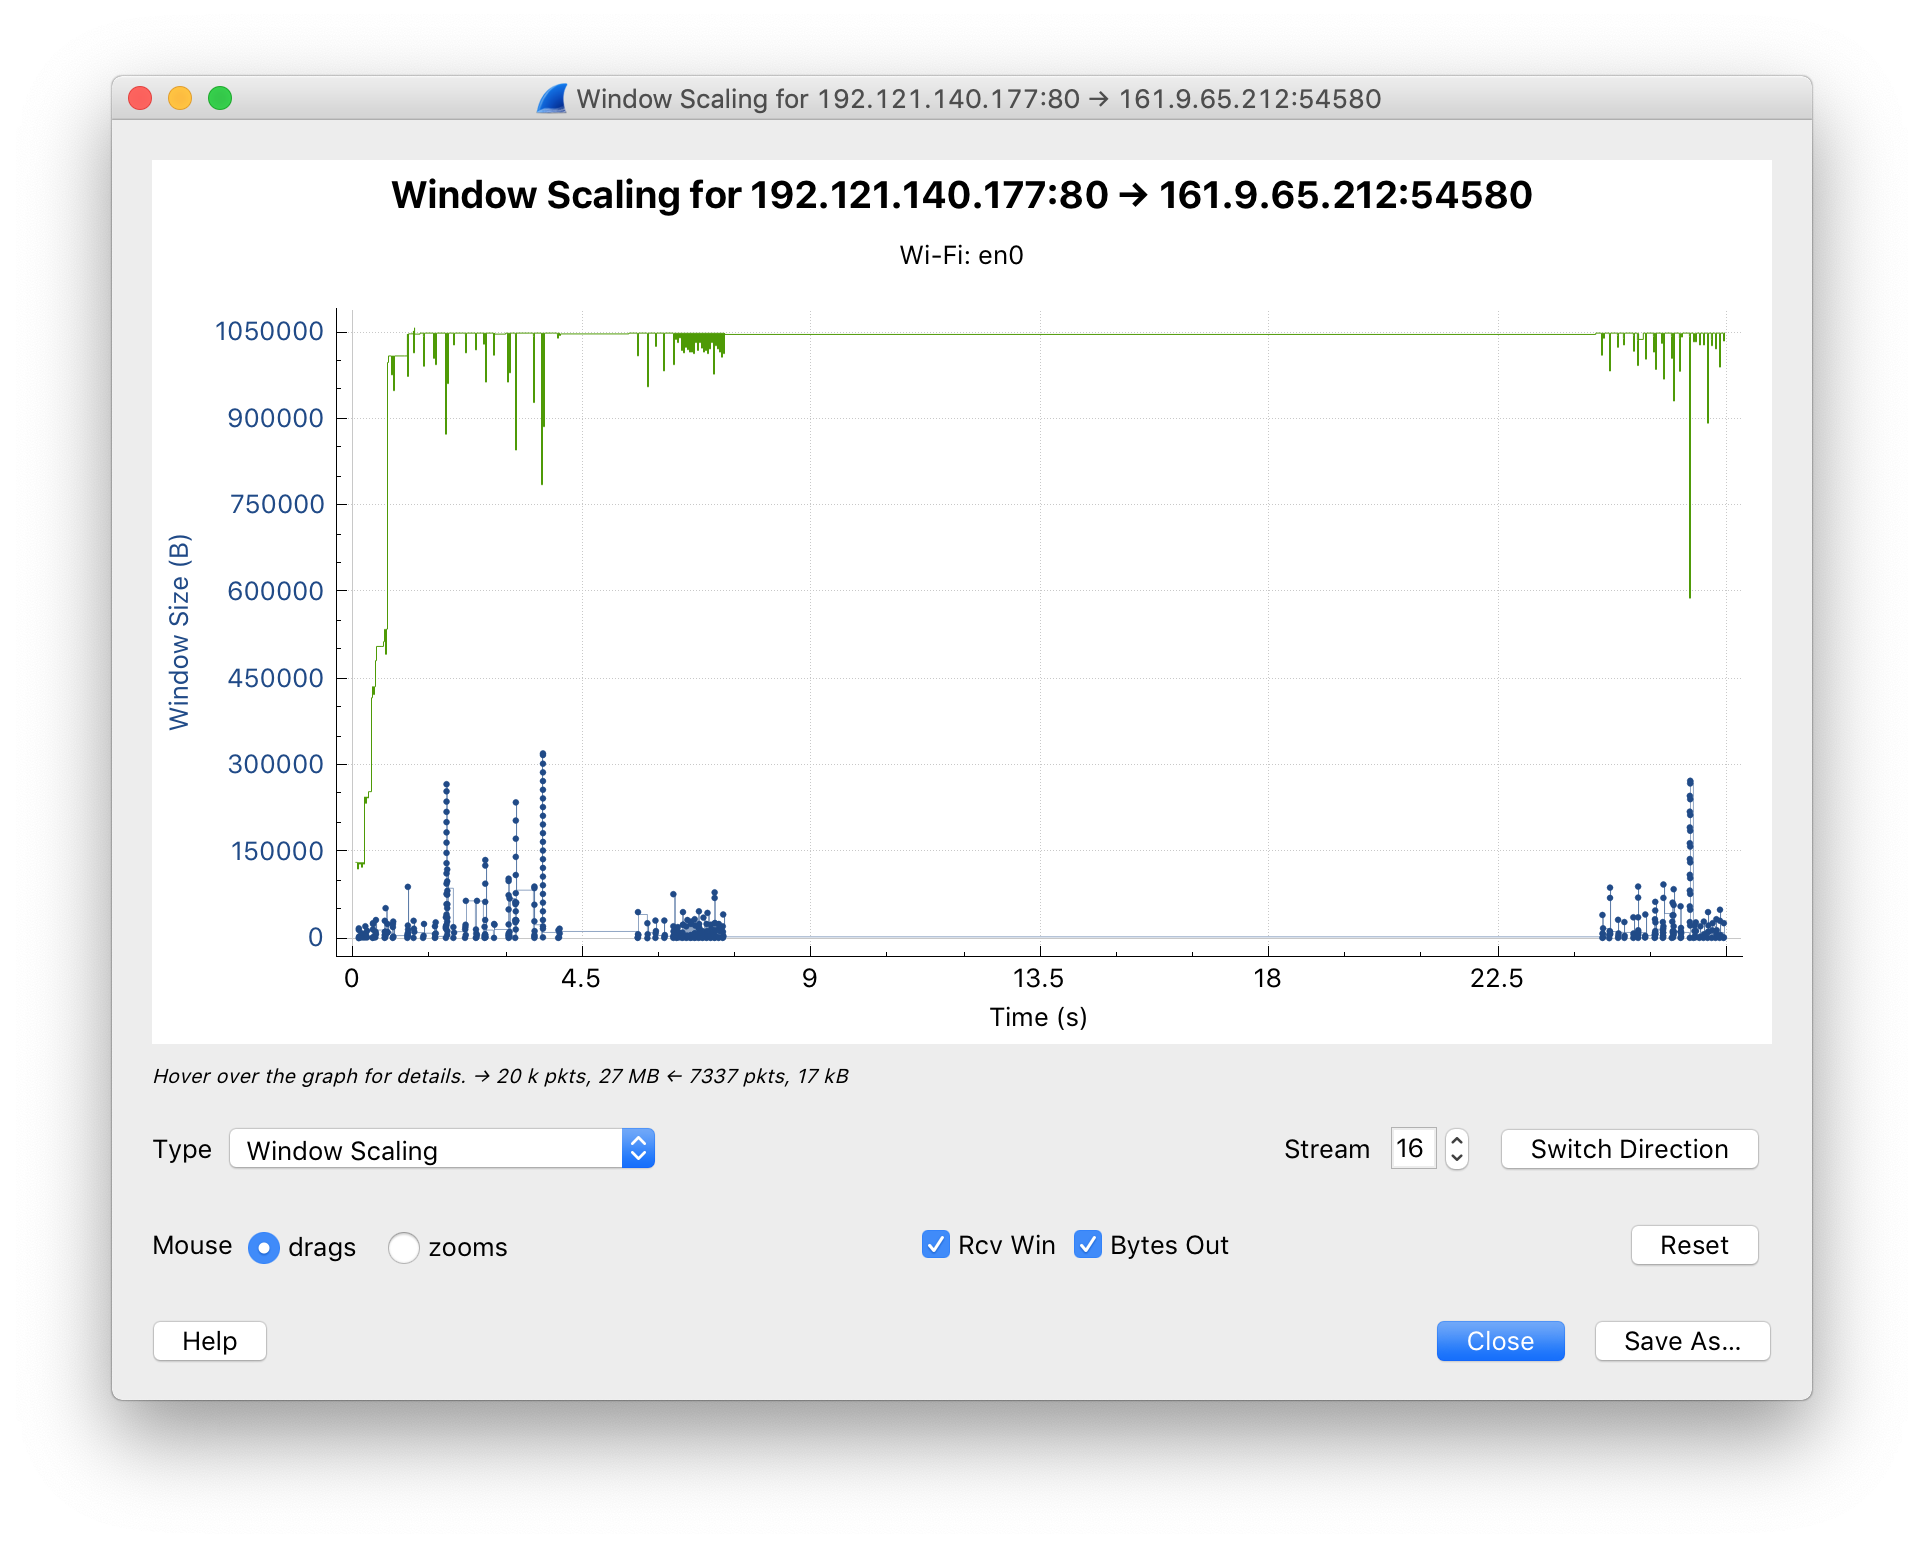
\includegraphics[width=0.7\linewidth]{window_scale2}
		\caption{Window Scaling for server to client}
	\end{figure}

	\clearpage
	
	\question{4}{File Transfer (20 Points)}
	
	Download a file on your browser and try to capture ftp packets over Wireshark. If you can't capture any, what may be the reason for that? Try the process with the link given, "ftp://speedtest.tele2.net/", and take a screenshot of an ftp packet. Interpret the steps you covered during the file transfer process.
	
	\begin{figure}[H]
		\centering
		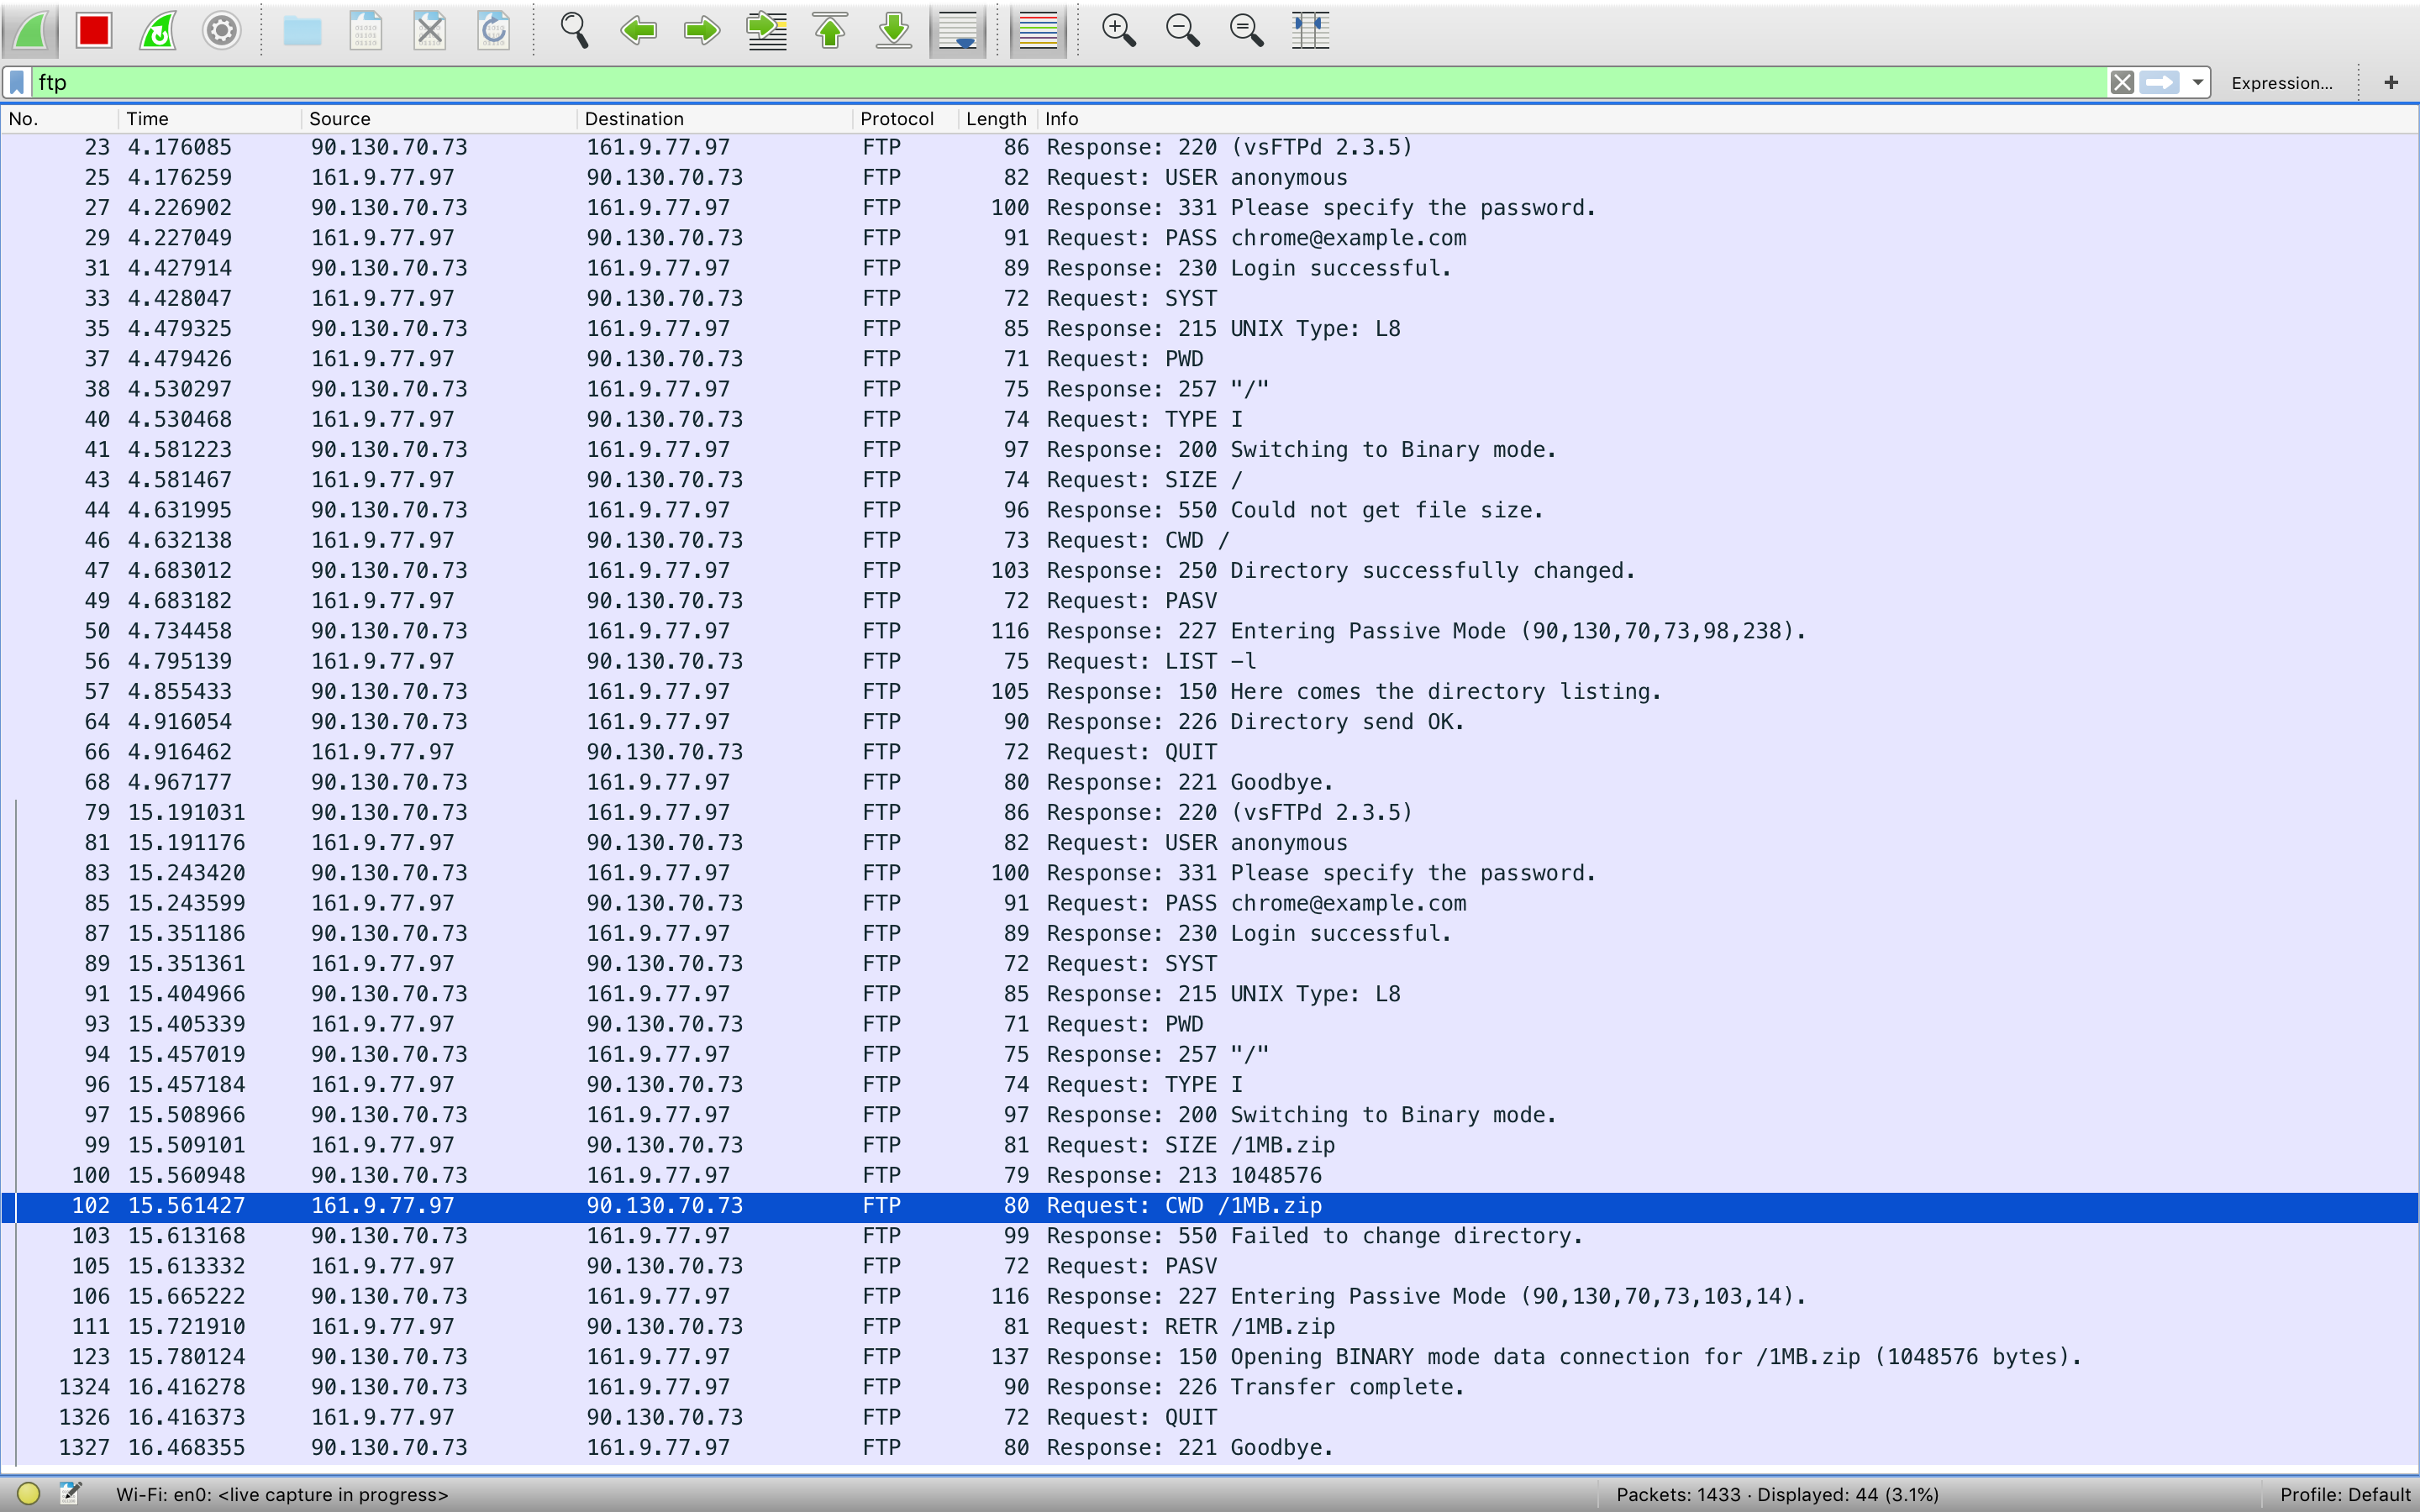
\includegraphics[width=1\linewidth]{ftp}
		\caption{FTP Packet Diagram captured by Wireshark}
	\end{figure}

	There are two ftp sessions stated in Figure 10. At every session user should send its username using the command "USER username" (i.e. frames no: 25, and 81 in Figure 10). Then the server wants the client to specify the password. Because the client is anonymous, browsers sends a sample password automatically. After a successfull login, the client requests the system type with the command "SYST", and the server responds the relevant information. PWD command is used to get the current directory, and CWD is used to change the working directory. To download a file from the server, the client sends the command "RETR filepath" to the server (frame no: 111), after that server broadcasts the file. At the end, the client send "QUIT" command in order to close connection, the server responds that request with "221 Goodbye" command.  
	
	\clearpage
	
	\question{5}{Protocol Analysis (20 Points)}
	
	\part{a} How many different traffic protocols do you capture in Wireshark? Please give them in a list.

	\begin{enumerate}
		\item Transmission Control Protocol (TCP)
		\item User Datagram Protocol (UDP)
		\item Transport Layer Security (TLSv1.2)
		\item Dynamic Host Configuration Protocol (DHCP)
		\item Extensible Authentication Protocol (EAP)
		\item Extensible Authentication Protocol over LAN (EAPOL)
		\item Address Resolution Protocol (ARP)
		\item Domain Name System (DNS)
		\item Internet Control Message Protocol (ICMPv6)
		\item Internet Group Management Protocol (IGMPv3, and IGMPv6)
		\item Multicast DNS (MDNS)
		\item NetBIOS Name Service (NBNS)
		\item Simple Service Discovery Protocol (SSDP)
		\item File Transfer Protocol (FTP)
	\end{enumerate}


	\part{b} What are the specific protocol numbers of transport layer protocols (TCP, UDP, and ICMP)? Please provide screenshots from Wireshark to show them in packet headers. \\
		
		\begin{figure}[H]
			\centering
			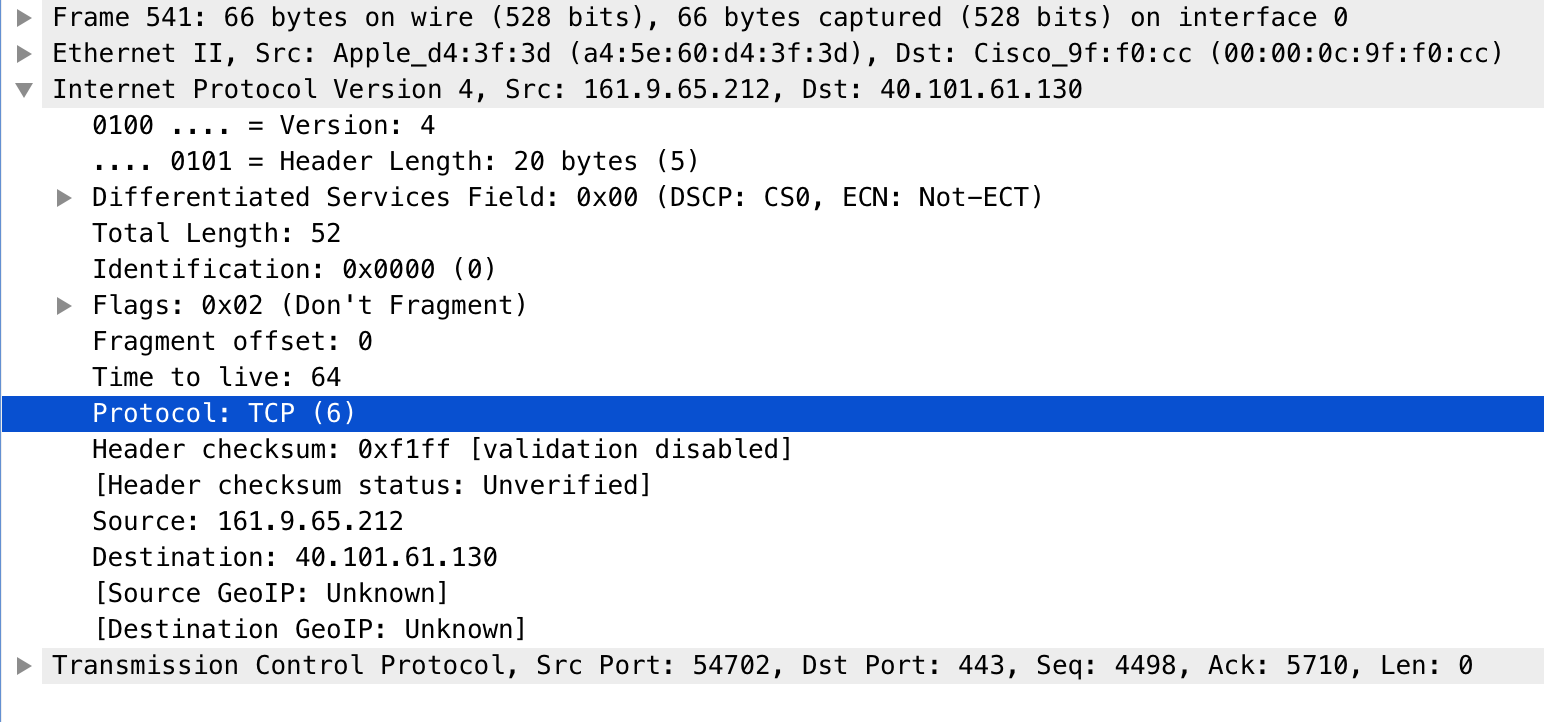
\includegraphics[width=0.9\linewidth]{tcp}
			\caption{TCP Number}
		\end{figure}
	
		\begin{figure}[H]
			\centering
			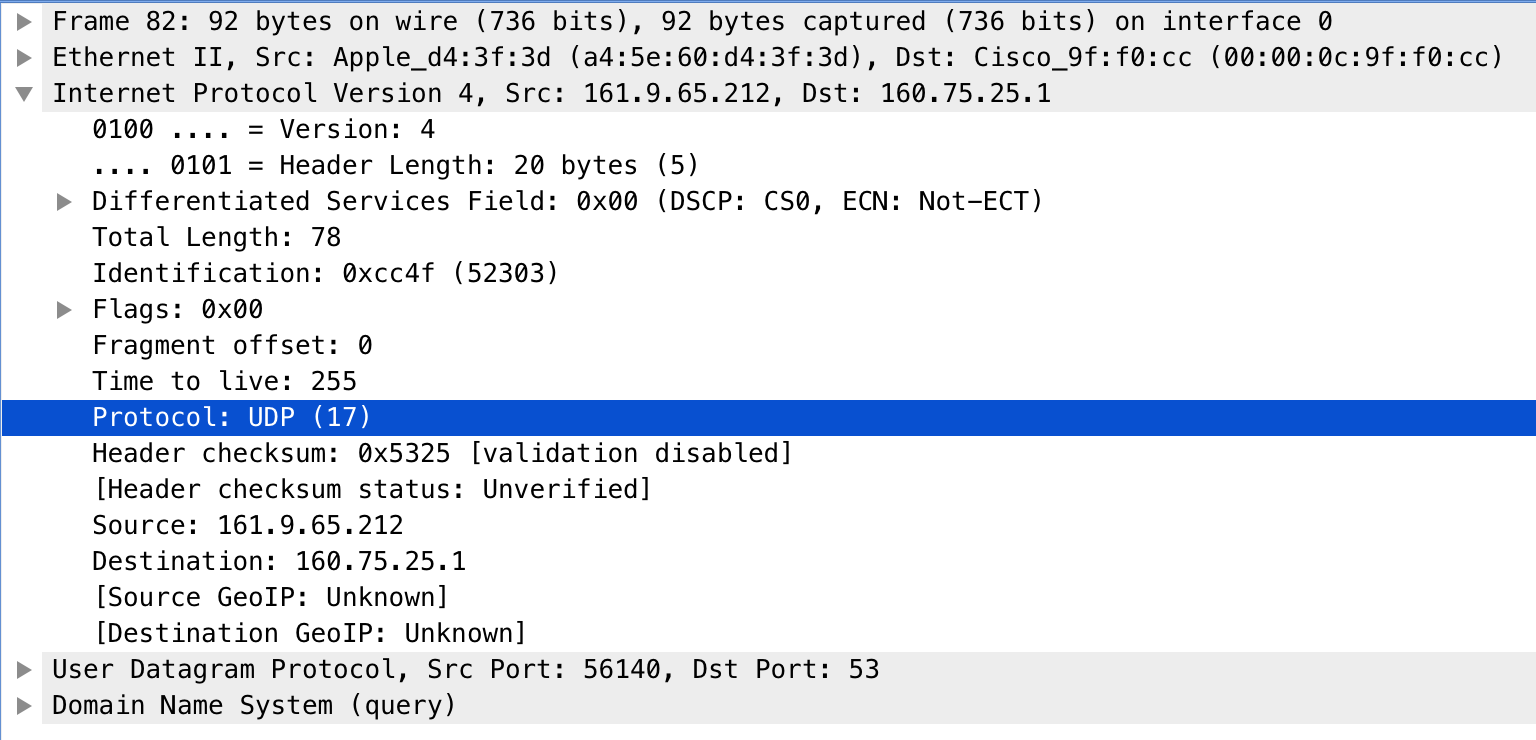
\includegraphics[width=0.9\linewidth]{udp}
			\caption{UDP Number}
		\end{figure}

		\begin{figure}[H]
			\centering
			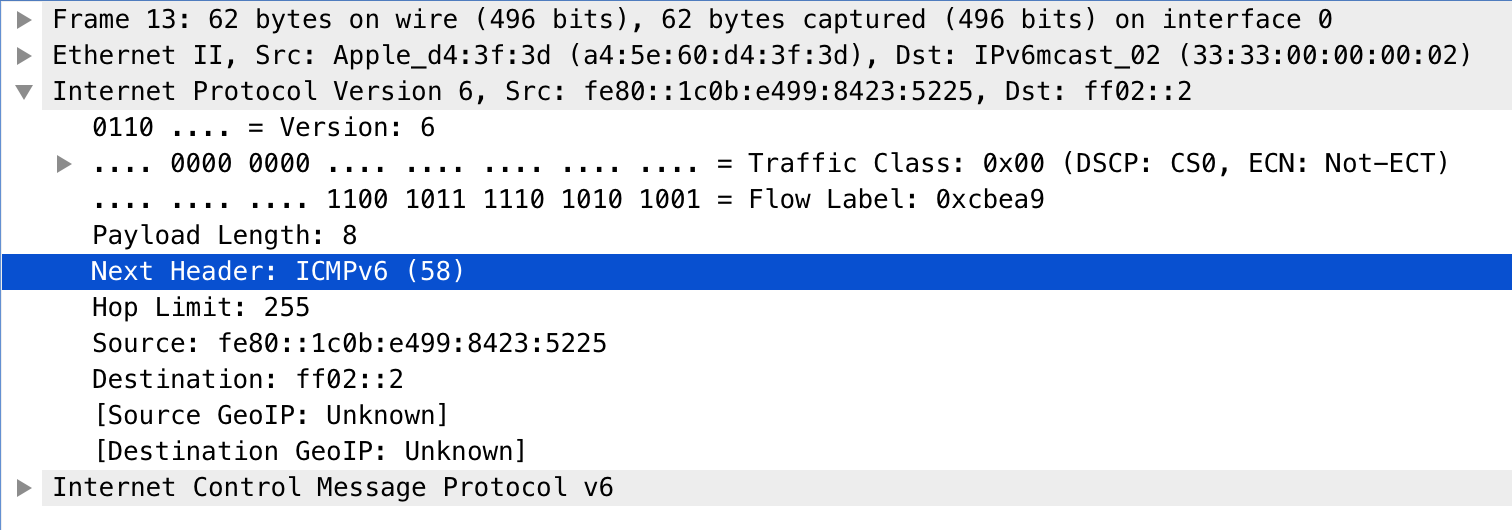
\includegraphics[width=0.9\linewidth]{icmp}
			\caption{ICMP Number}
		\end{figure}
		
\end{document}
